
El desarrollo de la Teoría de Conjuntos por Georg Cantor, aunado a la evolución del pensamiento matemático del siglo XIX, dio pie a una clase de razonamientos lógicos que hoy llamamos \textbf{argumentos diagonales}.

Estos argumentos revelan propiedades estructurales profundas mediante mecanismos de autorreferencia. A fin de ilustrar la esencia de este procedimiento, comenzaremos mostrando uno de los ejemplos más conocidos: la demostración de que los números reales son más grandes que los números naturales.


\begin{teo*}[Teorema de la Diagonal de Cantor]
El intervalo real unitario $(0,1)$ no es numerable. Es decir, no existe una biyección $\ff{\phi}{\N}{(0,1)}$.
\end{teo*}

\begin{proof}
Procederemos por reducción al absurdo. Supongamos que el conjunto es numerable y que, por tanto, existe una biyección $\phi$ que nos permite ennumerar los elementos del intervalo como una sucesión $x_1, x_2, x_3, \dots$, donde $x_n = \phi(n)$.

Podemos representar cada número $x_n$ mediante su expansión decimal única:
\begin{align*}
    x_1 &= 0.a_{11} a_{12} a_{13} a_{14} \dots \\
    x_2 &= 0.a_{21} a_{22} a_{23} a_{24} \dots \\
    x_3 &= 0.a_{31} a_{32} a_{33} a_{34} \dots \\
    &\vdotswithin{=} \\
    x_n &= 0.a_{n1} a_{n2} a_{n3} a_{nn} \dots 
\end{align*}
Buscamos encontrar un número real $y \in (0,1)$ que no se encuentre en dicha lista. Para ello, definimos $y = 0.d_1d_2d_3\dots$, donde los dígitos $d_n$ están dados por la siguiente regla:
\[
    d_n = \begin{cases} 
    1 & \text{si } a_{nn} \neq 1 \\
    2 & \text{si } a_{nn} = 1 
    \end{cases}
\]
Observemos que, dada esta regla, para cualquier índice $n \in \N$, el $n$-ésimo dígito de nuestro nuevo número $y$ difiere del $n$-ésimo dígito del número $x_n$ de la lista (es decir, $d_n \neq a_{nn}$). 

Esto implica necesariamente que $y \neq x_n$ para todo $n$. Sin embargo, $y$ es un número real bien definido con expansión decimal de unos y dos, por lo que $y \in (0,1)$. Por tanto, hemos encontrado un número en el intervalo $(0,1)$ que no está en la imagen de $\phi$, contradiciendo la hipótesis de que $\phi$ era sobreyectiva. Por lo tanto, concluimos que el intervalo $(0,1)$ no es numerable.
\end{proof}

Podemos observar en la demostración anterior que, para construir el elemento $y$, recurrimos explícitamente a la diagonal principal de la matriz; es decir, nos fijamos en los términos de la forma $a_{nn}$.

\begin{center}
\tikzset{every picture/.style={line width=0.75pt}}

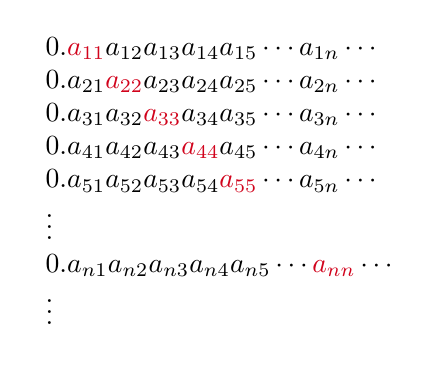
\begin{tikzpicture}[x=0.75pt,y=0.75pt,yscale=-1,xscale=1]
% Text Node
\draw (215,31.4) node [anchor=north west][inner sep=0.75pt]    {$ \begin{array}{l}
0.\textcolor[rgb]{0.82,0.01,0.11}{a_{11}} a_{12} a_{13} a_{14} a_{15} \cdots a_{1n} \cdots \\
0.a_{21}\textcolor[rgb]{0.82,0.01,0.11}{a_{22}} a_{23} a_{24} a_{25} \cdots a_{2n} \cdots \\
0.a_{31} a_{32}\textcolor[rgb]{0.82,0.01,0.11}{a_{33}} a_{34} a_{35} \cdots a_{3n} \cdots \\
0.a_{41} a_{42} a_{43}\textcolor[rgb]{0.82,0.01,0.11}{a_{44}} a_{45} \cdots a_{4n} \cdots \\
0.a_{51} a_{52} a_{53} a_{54}\textcolor[rgb]{0.82,0.01,0.11}{a_{55}} \cdots a_{5n} \cdots \\
\vdots \\
0.a_{n1} a_{n2} a_{n3} a_{n4} a_{n5} \cdots \textcolor[rgb]{0.82,0.01,0.11}{a_{nn}} \cdots \\
\vdots 
\end{array}$};
\end{tikzpicture}
\end{center}

La clave del argumento reside en el uso de esta información diagonal para definir un objeto que difiere sistemáticamente de todos los elementos listados. Observemos que el éxito de la construcción depende de la capacidad de \enquote{invertir} el valor encontrado en la diagonal. El apelar a esta estructura es lo que conocemos hoy como \textbf{argumento diagonal}.

Este argumento es generalizable y trasciende la geometría de una matriz infinita. En muchos contextos, la diagonal no es tan visible, pero el mecanismo subyacente es el mismo: la \textbf{autorreferencia}. 

Si trasladamos este argumento a la Teoría de Conjuntos intuitiva, sustituyendo la numeración por la relación de pertenencia, el argumento diagonal, en vez de producir un \enquote{nuevo elemento}, revela una contradicción en la estructura misma de la teoría. Esta contradicción fue descubierta por Bertrand Russell en 1901, y es conocida como la \textbf{Paradoja de Russell}. 

\subsection*{La Paradoja de Russell}

La Paradoja de Russell concierne a la ahora llamada \textit{Teoría Intuitiva de Conjuntos}, como fue inicialmente concebida por Georg Cantor. Esta teoría incial se fundamentaba en el principio de que cualquier propiedad lógica define un conjunto. Por ejemplo, la propiedad de ser un número par da pie al conjunto $A=\{2k\,|\, k\in \mathbb{N}\}$. Con esto en mente, para visualizar el problema necesitamos considerar conjuntos que puedan pertenecerse a sí mismos. Por ejemplo, el conjunto definido por la propiedad de \enquote{ser una idea} es, en sí mismo, una idea, y por lo tanto pertenece a sí mismo.

Consideremos el conjunto $R$, definido como la colección de todos los conjuntos que \textbf{no} son elementos de sí mismos:
\[R = \{X \mid X \notin X\}\]
Podemos entonces formular la siguiente pregunta: ¿Se pertenece $R$ a sí mismo?
Ante esto, tenemos dos posibilidades:
\begin{enumerate}
    \item $R \in R$. En este caso, tenemos que debe cumplir la condición que define al conjunto, es decir, tenemos $R \notin R$.
    \item $R \notin R$. En este otro caso, tenemos que cumple la propiedad que define a $R$ por lo que debe pertenecer al conjunto, es decir, $R \in R$.
\end{enumerate}
En ambos casos llegamos a la contradicción:
\[R \in R \iff R \notin R\]
Este resultado evidencia que la teoría intuitiva es inconsistente: no puede ser el caso que cualquier propiedad defina un conjunto. De permitirlo, el edificio lógico de la teoría se derrumbaría.

Ahora bien, hemos afirmado que en el corazón de esta paradoja reside la \textbf{autorreferencia} y que se trata de un argumento diagonal. La autoreferencia está presente para llegar a la Paradoja. Sin embargo, en la formulación anterior no construimos ninguna matriz ni apelamos a la diagonal. ¿Cómo es entonces que este ejemplo cae en un \enquote{argumento diagonal} como el que observamos con Cantor?

Imaginemos, conforme a la teoría intuitiva, que podemos enlistar \enquote{todos los conjuntos existentes}. Organicémoslos tanto vertical como horizontalmente para formar una tabla como la siguiente:

\begin{center}
$ \begin{matrix} 
& A & B & C & D & \dots \\
A & \cdot & \cdot & \cdot & \cdot & \\
B & \cdot & \cdot & \cdot & \cdot & \\
C & \cdot & \cdot & \cdot & \cdot & \\
\vdots & & & & & \ddots
\end{matrix} $
\end{center}

Asignemos valores de $1$ y $0$ de la siguiente forma: pondremos un $1$ si el conjunto de la fila pertenece al conjunto de la columna, y un $0$ en caso contrario. Supongamos, por ejemplo, que $A \notin A$ y $A \in B$. Los valores resultantes serían entonces $0$ y $1$, respectivamente. Nuestra matriz de pertenencia podría entonces lucir así:


\begin{center}
\tikzset{every picture/.style={line width=0.75pt}}

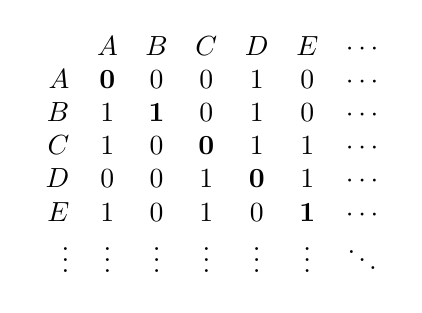
\begin{tikzpicture}[x=0.75pt,y=0.75pt,yscale=-1,xscale=1]
% Text Node
\draw (215,31.4) node [anchor=north west][inner sep=0.75pt]    {$
\begin{array}{rcccccc}
    & A & B & C & D & E & \cdots \\
  A & \mathbf{0} & 0 & 0 & 1 & 0 & \cdots \\
  B & 1 & \mathbf{1} & 0 & 1 & 0 & \cdots \\
  C & 1 & 0 & \mathbf{0} & 1 & 1 & \cdots \\
  D & 0 & 0 & 1 & \mathbf{0} & 1 & \cdots \\
  E & 1 & 0 & 1 & 0 & \mathbf{1} & \cdots \\
  \vdots & \vdots & \vdots & \vdots & \vdots & \vdots & \ddots
\end{array}
$};
\end{tikzpicture}
\end{center}



Al igual que en el teorema anterior, nuestra atención se centra en la \textbf{diagonal principal} que hemos resaltado. Las entradas con valor $0$ en la diagonal corresponden a los conjuntos $X$ tales que $X \notin X$.
La definición de $R$ es precisamente la instrucción de tomar esos casos: $R$ se define \enquote{invirtiendo} la diagonal principal.
\[ X \in R \iff \text{Diagonal}(X, X) = 0 \]
Dado que $R$ es un conjunto dentro de esta teoría, debe ocupar algún lugar en la lista, es decir, la fila $R$. ¿Qué valor tiene $R$ en su propia intersección diagonal? Por construcción, debe tener el valor opuesto al que tiene en la diagonal. Es decir, el valor en $(R, R)$ debe ser $0$ si y solo si es $1$.

Esta visualización confirma que la paradoja es estructuralmente idéntica al argumento de Cantor: el problema surge al intentar introducir dentro de la matriz un objeto definido por la negación de la diagonal de dicha matriz.

Siguiendo estos casos de autorreferencia, el más célebre y con mayor peso filosófico es indudablemente el \textbf{Primer Teorema de Incompletitud de Gödel}. Un planteamiento y demostración rigurosa de este teorema ocuparía demasiado espacio y se saldría de los objetivos de esta introducción. Por ello, nos limitaremos a dar un esbozo que sigue la línea argumental presentada por el propio Gödel en \cite{gdl}, resaltando cómo es, en el fondo, otro argumento diagonal.

\subsection*{El Teorema de Incompletitud de Gödel}


Los sistemas formales que fundamentan la matemática moderna, tales como los Axiomas de Peano o la Teoría de Conjuntos de Zermelo-Fraenkel, poseen la capacidad expresiva suficiente para construir la aritmética básica de los números naturales. La expectativa histórica, liderada por el programa de Hilbert, era que estos sistemas fueran capaces de decidir la verdad o falsedad de cualquier proposición formulada en su lenguaje.

Sin embargo, estos sistemas presentan limitaciones internas fundamentales respecto a lo que pueden demostrar. Gödel probó que, si estos sistemas son \textbf{consistentes} (que no poseen contradicciones), existen  entonces proposiciones en dichos sistemas que son \textit{indecidibles}; es decir, enunciados que el sistema no es capaz de demostrar como verdaderos ni refutar como falsos.

Podría pensarse que la solución radica en añadir estas proposiciones como nuevos axiomas. No obstante, esto no resuelve el problema estructural: en el nuevo sistema ampliado surgirían inevitablemente nuevas proposiciones indecidibles. Este fenómeno de incompletitud no es exclusivo de los dos sistemas mencionados; como veremos en el Capítulo 3, una clase extensiva de sistemas formales sufren de esta limitación.


En el corazón de este problema yace, nuevamente, la autorreferencia. Construimos una proposición que afirma algo sobre su propia indemostrabilidad. Para formalizar esto, Gödel tuvo que idear una manera de que la aritmética \enquote{hablara de sí misma}.

La idea central y genial de Gödel fue trasladar el problema de la autorreferencia al lenguaje de la aritmética. Para ello, ideó un método de codificación (conocido como \textit{numeración de Gödel}) que asigna a cada fórmula $\phi$ del sistema un número natural único, denotado por $\ulcorner \phi \urcorner$. Esto permite que la aritmética \enquote{hable} de sus propias fórmulas.

Gracias a esta codificación, la propiedad metamatemática \enquote{$y$ es una demostración de $x$} se puede expresar como una relación aritmética, llamémosla $\dems(x,y)$. A partir de aquí, podemos definir el concepto de ser demostrable como 

\begin{center}
    
$x$ es demostrable $ \iff \exists y \dems(x,y).$

\end{center}
Nace de aquí la diagonal como en los otros dos ejemplos. Gödel definió una función de sustitución $s(n, m)$, que calcula el código de la fórmula resultante al tomar la fórmula con código $n$ y reemplazar su variable libre por el número $m$, es decir, 
\[ s(\ulcorner \phi(x) \urcorner, m) = \ulcorner \phi(m) \urcorner. \]
Esta función $s$ es la herramienta que nos permite \enquote{caminar por la diagonal}: si evaluamos $s(n, n)$, estamos pidiéndole intrínsecamente a la fórmula número $n$ que hable del número $n$. Es el análogo aritmético de mirar la entrada $(n,n)$ en la matriz del argumento de la diagonal de Cantor o en la matriz que visualizamos de pertencencia para la Paradoja de Russell.

Ahora, consideremos la siguiente fórmula:
\[ P(x) := \neg \dems( s(x, x) ). \]
Sea $k$ el número de Gödel de esta fórmula, es decir, $k = \ulcorner P(x) \urcorner$. Si evaluamos ahora la diagonal en este punto (calculamos $P(k)$), obtenemos una sentencia $G$ tal que:
\[ G \iff \neg \dems( s(k, k) ) \]
Pero por definición de nuestra función de sustitución, $s(k, k)$ es precisamente el código de $G$. Es decir, $\ulcorner G \urcorner = s(k, k)$. Sustituyendo esto, llegamos a:
\[ G \iff \neg \dems( \ulcorner G \urcorner ) \]
Esta sentencia $G$ afirma, esencialmente: \enquote{yo no soy demostrable}.

Si el sistema es consistente, no puede demostrar falsedades, por lo que no puede demostrar $G$ (ya que si lo hiciera, $G$ sería falsa). Pero al no poder demostrarla, lo que $G$ afirma es verdad. Tenemos entonces una sentencia que es verdadera pero no demostrable dentro del sistema.

Para visualizar la naturaleza diagonal de este argumento, podemos recurrir a la misma representación matricial que utilizamos con Cantor y Russell.

Imaginemos una lista enumerada de todas las fórmulas posibles con una variable libre en el lenguaje de la aritmética: $\phi_0(x), \phi_1(x), \phi_2(x), \dots$.
En las columnas, colocamos los números naturales que pueden servir como argumentos para estas fórmulas.

Definamos el valor de la entrada $(n, m)$ en esta matriz como $1$ si el sistema demuestra que la fórmula $\phi_n$ es verdadera para el número $m$ (es decir, si $\vdash \phi_n(m)$), y $0$ en caso contrario.

\begin{center}
\tikzset{every picture/.style={line width=0.75pt}}

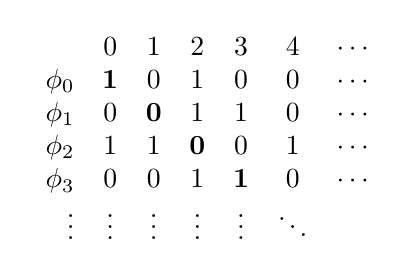
\begin{tikzpicture}[x=0.75pt,y=0.75pt,yscale=-1,xscale=1]
% Text Node
\draw (215,31.4) node [anchor=north west][inner sep=0.75pt]    {$
\begin{array}{rcccccc}
    & 0 & 1 & 2 & 3 & 4 & \cdots \\
  \phi_0 & \mathbf{1} & 0 & 1 & 0 & 0 & \cdots \\
  \phi_1 & 0 & \mathbf{0} & 1 & 1 & 0 & \cdots \\
  \phi_2 & 1 & 1 & \mathbf{0} & 0 & 1 & \cdots \\
  \phi_3 & 0 & 0 & 1 & \mathbf{1} & 0 & \cdots \\
  \vdots & \vdots & \vdots & \vdots & \vdots & \mathbf{\ddots} & 
\end{array}
$};
\end{tikzpicture}
\end{center}

Nuevamente, nuestra atención se dirige a la \textbf{diagonal principal}. Esta diagonal representa si es demostrable cada fórmula cuando es aplicada a su propio número de código o dicho de otra forma: la entrada $(n, n)$ en la matriz nos dice si $\vdash \phi_n(n)$.

La sentencia indecidible de Gödel, $G$, se construye esencialmente definiendo una nueva fila (una nueva fórmula) que \enquote{invierte} los valores de esta diagonal. La fórmula $G(x)$ está diseñada para comportarse como la negación de la diagonal:
\[ G(n) \text{ es verdadera} \iff \text{la entrada} (n,n) \text{de la matriz es } 0 \]
Como $G$ es una fórmula válida en el sistema, debe aparecer en algún lugar de la lista de filas, digamos en la fila $k$. La contradicción (o en este caso, la indecidibilidad) surge al preguntar por el valor de la intersección $(k, k)$. La fórmula debe negar su propio valor en la diagonal, llegando así a que es verdadera si y solo si no es demostrable.

A pesar de que los tres ejemplos expuestos difieren sustancialmente en su contenido proposicional —el primero trata sobre cardinalidades infinitas, el segundo sobre inconsistencias en la teoría intuitiva de conjuntos y el tercero sobre las limitaciones deductivas de la aritmética—, todos comparten un método subyacente idéntico en esencia. En cada caso, la motivación principal surge de una noción de \textbf{autorreferencia} que es \enquote{transmitida} a la demostración matemática.

 Es precisamente este rasgo autorreferencial el que ha rodeado de un halo de misticismo y especulación filosófica a los Teoremas de Incompletitud de Gödel y, en general, a muchos resultados obtenidos mediante argumentos diagonales. Surge entonces una interrogante natural: si el germen de la autorreferencia puede incrustarse en el corazón de las matemáticas mediante un mecanismo tan simple, ¿acaso hay una noción más allá de lo científico que las limite?

Esta inquietud fue popular durante gran parte del siglo XX, impulsada por la crisis de los fundamentos. Sin embargo, en 1969, William F. Lawvere publicó unas notas que, silenciosa pero contundentemente, derrumbarían este misticismo. En su artículo \textit{Diagonal Arguments and Cartesian Closed Categories}, Lawvere observó que todos estos argumentos no son sino consecuencias naturales de trabajar en tipos particulares de estructuras categóricas. En sus propias palabras:

\begin{quote}
The original aim of this article was to demystify the incompleteness theorem of Gödel and the truth-definition theory of Tarski by showing that both are consequences of some very simple algebra in the cartesian-closed setting.
\end{quote}

El aporte de Lawvere es fundamental: logró unificar en un solo esquema formal algunos de los resultados de imposibilidad más importantes del siglo pasado. Más adelante, este hallazgo sería conocido como el \textbf{Teorema del Punto Fijo de Lawvere}, uniéndose a la vasta familia de teoremas de punto fijo que abundan en diversas áreas de la matemática. 

No obstante, y a pesar de su trascendencia unificadora, este teorema permanece sorprendentemente poco difundido. Una posible explicación radica en que el lenguaje natural del resultado, la Teoría de Categorías, es una disciplina relativamente joven y, en ocasiones, ajena a la formación matemática tradicional. Por ello, existe un vacío en la literatura divulgativa y educativa respecto a este resultado. El presente trabajo nace de la intención de llenar ese vacío, presentando el Teorema del Punto Fijo de Lawvere de manera autocontenida y accesible, sin asumir conocimientos previos en Teoría de Categorías.

Como el presente trabajo es autocontenido, en el \textbf{Capítulo 1} nos enfocamos en introducir los conocimientos de Teoría de Categorías necesarios. Dado que no se trata de un curso extensivo de Teoría de Categorías, nos limitaremos a los conceptos indispensables para llegar al resultado deseado. El lector interesado en profundizar en esta teoría puede consultar \cite{Rie16}, \cite{Lei16} y \cite{Mac97}.

El \textbf{Capítulo 2} aborda el núcleo del trabajo: el \textbf{Teorema del Punto Fijo de Lawvere}. Presentamos una versión modernizada y una demostración más detallada que la original de Lawvere en \cite{Law06}. Es en este capítulo donde introducimos el concepto de \textit{categoría cartesiana cerrada}, enfatizando su papel crucial como el entorno donde estos argumentos diagonales ocurren. Además, veremos aquí también la contrapositiva del teorema, que es en esencia el resultado que da pie a estos argumentos diagonales.

El \textbf{Capítulo 3} explora las aplicaciones del teorema a través de diversas áreas de la matemática. Este es el capítulo más extenso, pues el interés principal de este trabajo es demostrar la utilidad y extensividad del resultado de Lawvere. 

El \textbf{Capítulo 4} presenta las conclusiones del trabajo.

La bibliogafía usada para esta tesis se podrá encontrar al final de la misma.
